\chapter{Derivadas parciales}

\newpage
\section{Derivadas parciales}

\subsection{Derivadas parciales de primer orden}

\subsection{Derivadas parciales de orden superior}

\subsection{Diferenciabilidad}

\subsection{Derivada direccional}

\subsection{Gradiente}

\subsection{Regla de la cadena}

\subsection{Derivación implícita}

\newpage
\section{Planos tangentes}

\begin{definicion}[plano tangente]
    Sea $S$ una superficie definida por $z=f(x,y)$, y sea $P=(a,b,f(a,b))$ un punto de $S$. El plano tangente a $S$ en el punto $P$ es el plano que pasa por $P$ y es paralelo al plano tangente a la gráfica de $f$ en el punto $(a,b)$.
\end{definicion}

\begin{teorema}[ecuación del plano tangente]
    Sea $S$ una superficie definida por $z=f(x,y)$, y sea $P=(a,b,f(a,b))$ un punto de $S$. Si las derivadas parciales de $f$ existen en el punto $(a,b)$, entonces el plano tangente a $S$ en el punto $P$ está dado por la ecuación:
    \[
    z-f(a,b)=\dfrac{\partial f}{\partial x}(a,b)(x-a)+\dfrac{\partial f}{\partial y}(a,b)(y-b).
    \]
\end{teorema}

\begin{figure}[H]
    \centering
    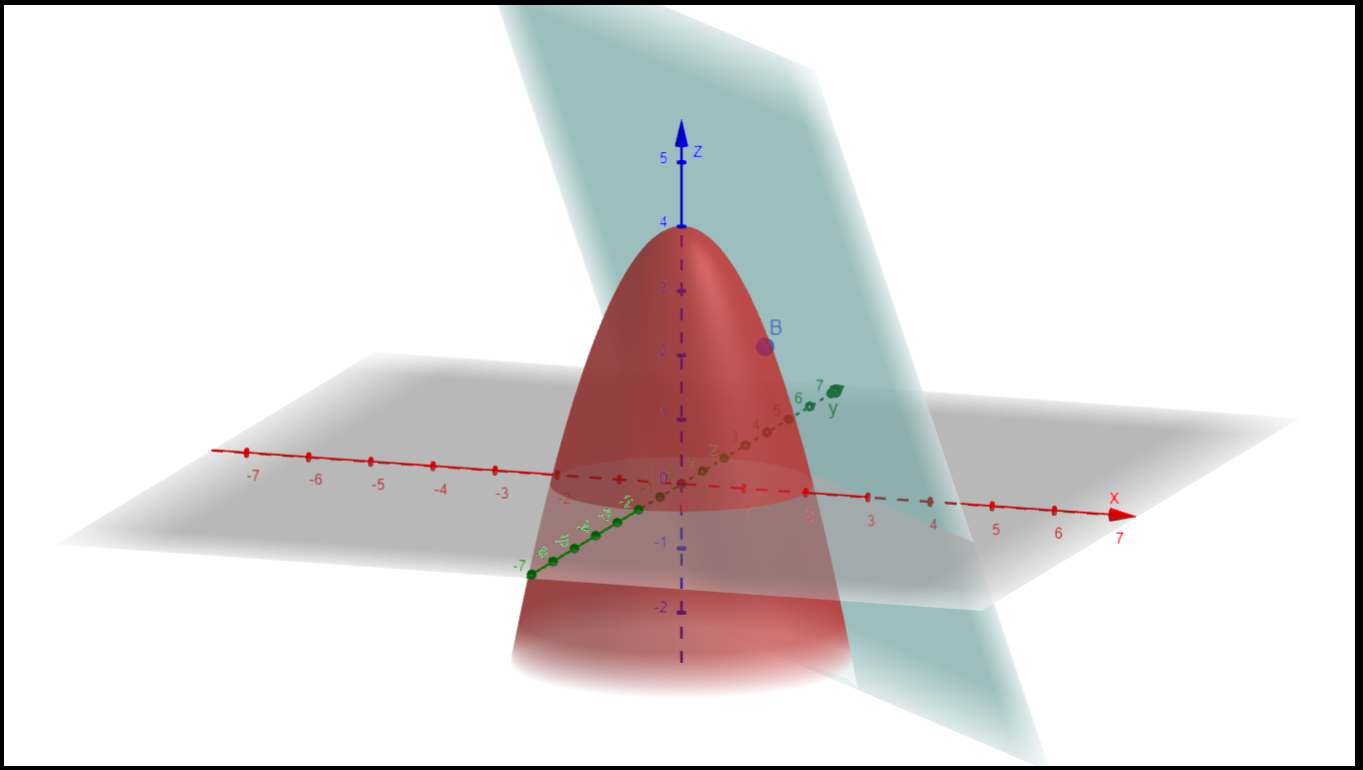
\includegraphics[width=1\textwidth]{C5.png}
    \caption{Gráfica de un plano tangente a un paraboloide.}
    \label{fig:plano_tangente_paraboloide}
\end{figure}

\newpage
\section{Rectas normales}

\newpage
\section{Máximos y mínimos}

\noindent
\begin{minipage}[t]{0.6\textwidth}
\hspace*{0.65cm}Si bien el desarrollo de métodos de optimización en cálculo es resultado de aportes de diferentes matemáticos a los largo de la historia, partiendo por Newton y Leibniz y pasando por eminencias como Euler, Lagrange y Bernoulli, hay otro matemático tal vez menos conocido pero cuyo nombre resonará con frecuencia en el estudio de esta unidad.\\

\hspace*{0.65cm}En el siglo XIX, el estudio de métodos de optimización se volvió más riguroso gracias al desarrollo de las derivadas segundas y la matriz Hessiana, ésta última, asociada al trabajo de Ludwig Otto Hesse.\\
\end{minipage}
\hfill
\begin{minipage}[t]{0.35\textwidth}
\vspace{-8mm}
\begin{figure}[H]
    \centering
    \fbox{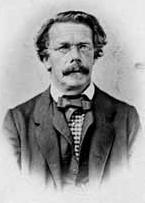
\includegraphics[width=4cm,height=5.5cm]{Ludwig_Otto_Hesse.jpg}}
    \caption{Retrato de Ludwig Otto Hesse. Fuente: Wikimedia Commons.}
    \label{fig:hesse}
\end{figure}
\end{minipage}

Ludwig Otto Hesse (1811-1874) fue un matemático alemán reconocido por sus trabajos en geometría analítica. Obtuvo su doctorado en la universidad de Königsberg (actual Kaliningrado), donde trabajó en superficies algebraicas dirigido por Jacobi. A lo largo de su vida realizó importantes contribuciones, como estudios analíticos de las redes de cónicas,ecuaciones de curvas en coordenadas tangenciales, geometría protectiva, entre muchas otras.



\newpage

\noindent
\begin{minipage}[t]{0.6\textwidth}
\hspace*{0.65cm}Recordemos que para encontrar los valores extremos de una funciuón de una variable $f:I \subset \mathbb{R} \mapsto \mathbb{R}, y=f(x)$; buscamos puntos donde la gráfica tenga tangente horizontal, para luego clasificarlos como máximos o mínimos.

\hspace*{0.65cm}Para el caso de una función de 2 variables $f:U \subset \mathbb{R}^2 \mapsto \mathbb{R}, z=f(x,y)$; el proceso es similar, pero ahora buscamos puntos donde la superficie tenga un plano tangente horizontal, paralelo al plano $XY$. Al igual que antes, estos serán puntos críticos que luego clasificaremos.
\end{minipage}
\hfill
\begin{minipage}[t]{0.35\textwidth}
\vspace{-0.4cm}
\begin{figure}[H]
    \centering
    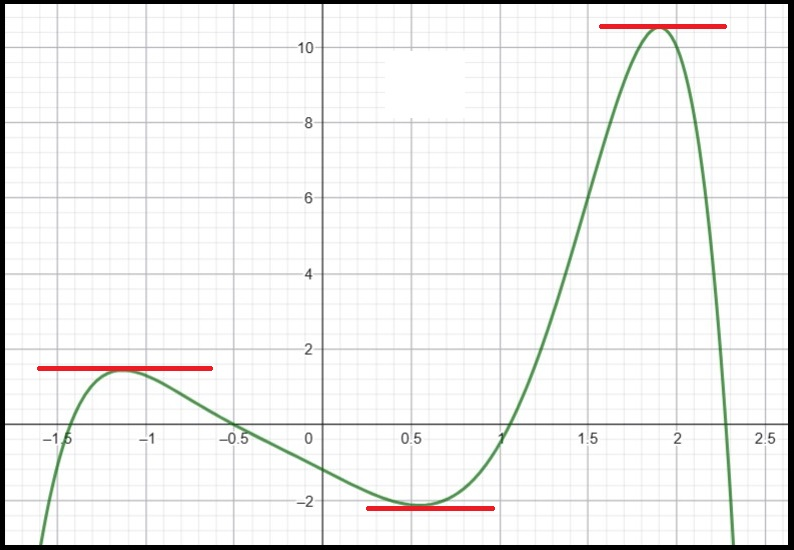
\includegraphics[width=1\textwidth]{C4.jpg}
    \caption{Gráfica de una función de una variable y las tangentes de sus puntos críticos.}
    \label{fig:tangentes_funcion_1_variable}
\end{figure}
\end{minipage}

\begin{definicion}[máximo relativo]
    Una función de dos variables $f(x,y)$ tiene un \textbf{máximo relativo} en el punto $(a,b)$ si existe un disco con centro $(a,b)$, tal que para todo punto $(x,y)$ en ese disco se cumple que $f(x,y)\leq f(a,b)$.
\end{definicion}

\begin{definicion}[mínimo relativo]
    Una función de dos variables $f(x,y)$ tiene un \textbf{mínimo relativo} en el punto $(a,b)$ si existe un disco con centro $(a,b)$, tal que para todo punto $(x,y)$ en ese disco se cumple que $f(x,y)\geq f(a,b)$.
\end{definicion}

Podemos entender este concepto de ``disco'' como una vecindad circular alrededor del punto $(a,b)$. Cuando trabajamos con funciones de una variable, esta vecindad era unidimensional, dada por: $0<|x-a|<\delta$. Para funciones de dos variables, esta vecindad se extiende a un área circular alrededor del punto $(a,b)$, definida por la condición $0<\sqrt{(x-a)^2+(y-b)^2}<\delta$.

Cuando se requiere generalizar este concepto a funciones de $n$ variables, se introduce el concepto de \textbf{bola}, que es la extensión n-dimensional del disco.

\begin{multicols}{2}
    \begin{figure}[H]
        \centering
        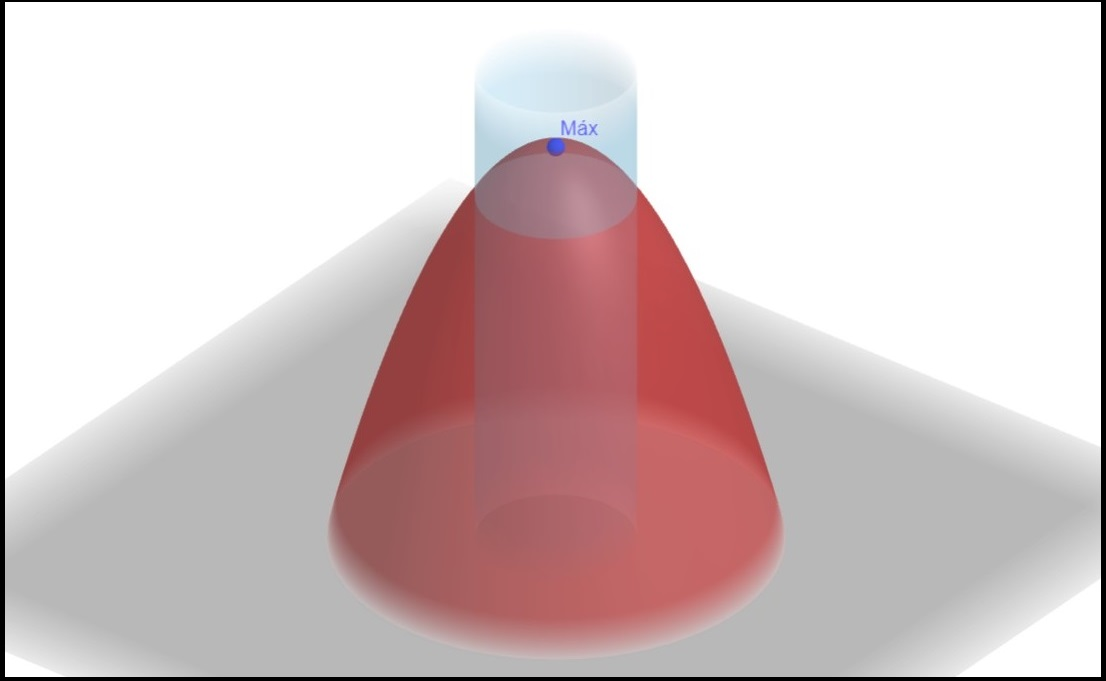
\includegraphics[width=5cm,height=5cm]{C6.jpg}
        \caption{Máximo relativo. La vecindad en torno a este punto se representa acotada por un cilindro.}
        \label{fig:maximo_relativo}
    \end{figure}
    \columnbreak
    \begin{figure}[H]
        \centering
        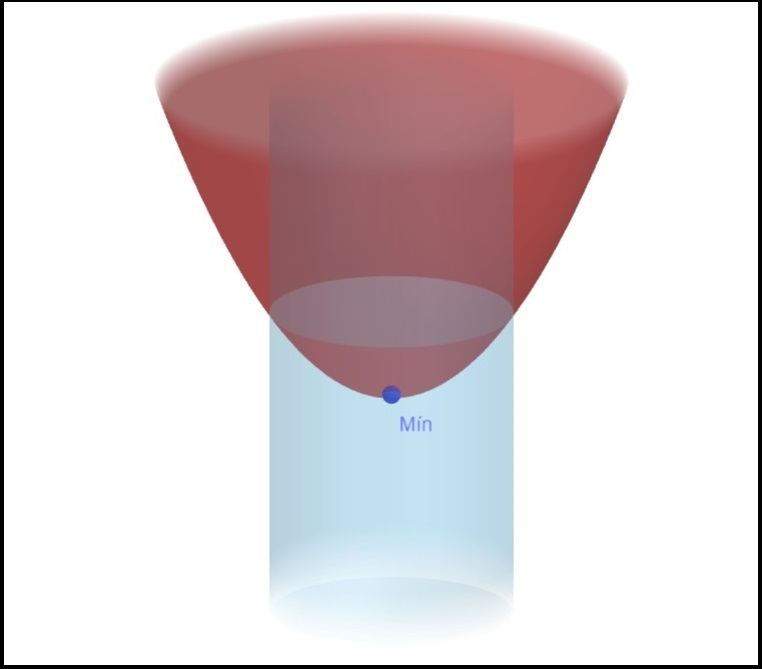
\includegraphics[width=5cm,height=5cm]{C7.jpg}
        \caption{Mínimo relativo. La vecindad en torno a este punto se representa acotada por un cilindro.}
        \label{fig:minimo_relativo}
    \end{figure}
\end{multicols}

\newpage

De manera similar a lo que ocurre con funciones de una variable, para encontrar los puntos críticos de una función de varias variables, es necesario que las derivadas parciales de primer orden se anulen. Esto se debe a que un plano tangente horizontal implica que la pendiente en ambas direcciones (x e y) es cero.

\begin{teorema}[condición necesaria para extremos relativos]
    Si $f$ tiene un máximo o mínimo relativo en el punto $(a,b)$ y las derivadas parciales de $f$ existen en dicho punto, entonces $\dfrac{\partial f}{\partial x}(a,b)=0$ y $\dfrac{\partial f}{\partial y}(a,b)=0$.
\end{teorema}

Una vez hayamos encontrado los puntos críticos, es decir, aquellos donde las derivadas parciales de primer orden se anulan, necesitamos un método para clasificarlos como máximos, mínimos o puntos de silla. Para esto, utilizaremos el siguiente teorema:

\begin{teorema}[prueba de la segunda derivada]
    Sea $f$ una función de dos variables con derivadas parciales de segundo orden continuas en un entorno de un punto crítico $(a,b)$, es decir, un punto donde $\dfrac{\partial f}{\partial x}(a,b)=0$ y $\dfrac{\partial f}{\partial y}(a,b)=0$. Definamos $D=f_{xx}(a,b)f_{yy}(a,b)-\left(f_{xy}(a,b)\right)^2$. Entonces:
    \begin{itemize}
        \item Si $D>0$ y $f_{xx}(a,b)>0$, entonces $f$ tiene un mínimo relativo en $(a,b)$.
        \item Si $D>0$ y $f_{xx}(a,b)<0$, entonces $f$ tiene un máximo relativo en $(a,b)$.
        \item Si $D<0$, entonces $f$ no tiene ni máximo ni mínimo relativo en $(a,b)$ (es decir, es un punto de silla).
        \item Si $D=0$, el test es inconcluso.
    \end{itemize}
\end{teorema}

El resultado $D$ se suele llamar el \textbf{discriminante} de la función $f$ en el punto crítico $(a,b)$, y es una medida de la curvatura de la función en ese punto. Si $D$ es positivo, la función tiene una curvatura similar a un paraboloide elíptico, lo que indica un máximo o mínimo relativo dependiendo del signo de $f_{xx}$. Si $D$ es negativo, la función tiene una curvatura similar a un paraboloide hiperbólico, lo que indica un punto de silla. Si $D$ es cero, la curvatura es degenerada y el test no puede determinar la naturaleza del punto crítico.

\newpage

Comencemos aplicando estos teorema con superficies donde resulte evidente la existencia de un punto extremo, como es el caso del paraboloide.

\begin{ejemplo}
    Dada la función $f(x,y)=x^2+y^2$, encontrar sus puntos críticos y clasificarlos.
\end{ejemplo}
\textbf{Solución:}
\begin{itemize}
    \item Primero, calculamos las derivadas parciales de primer orden, esto nos permitirá encontrar los puntos críticos:
    \[
\frac{\partial f}{\partial x} = 2x, \quad \frac{\partial f}{\partial y} = 2y.
    \]
    \item Para encontrar los puntos críticos, igualamos ambas derivadas parciales a cero:
    \[
2x = 0 \implies x = 0, \quad 2y = 0 \implies y = 0
    \]
    \item Por lo tanto, el único punto crítico es $(0,0)$.
    \item Ahora, calculamos las derivadas parciales de segundo orden, esto nos permitirá clasificar el punto crítico:
    \[
    f_{xx} = 2, \quad f_{yy} = 2, \quad f_{xy} = 0
    \]
    \item Calculamos $D$:
    \[
    D = f_{xx}f_{yy} - (f_{xy})^2 = (2)(2) - (0)^2 = 4 > 0
    \]
    \item Dado que $D > 0$ y $f_{xx} > 0$, concluimos que $f$ tiene un mínimo relativo en el punto $(0,0)$.
\end{itemize}

\begin{ejemplo}
    Dada la función $f(x,y)=-(x^2+y^2)$, encontrar sus puntos críticos y clasificarlos.
\end{ejemplo}

\textbf{Solución:}
\begin{itemize}
    \item Primero, calculamos las derivadas parciales de primer orden, esto nos permitirá encontrar los puntos críticos:
    \[
\frac{\partial f}{\partial x} = -2x, \quad \frac{\partial f}{\partial y} = -2y.
    \]
    \item Para encontrar los puntos críticos, igualamos ambas derivadas parciales a cero:
    \[
    -2x = 0 \implies x = 0, \quad -2y = 0 \implies y = 0
    \]
    \item Por lo tanto, el único punto crítico es $(0,0)$.
    \item Ahora, calculamos las derivadas parciales de segundo orden, esto nos permitirá clasificar el punto crítico:
    \[
    f_{xx} = -2, \quad f_{yy} = -2, \quad f_{xy} = 0
    \]
    \item Calculamos $D$:
    \[
    D = f_{xx}f_{yy} - (f_{xy})^2 = (-2)(-2) - (0)^2 = 4 > 0
    \]
    \item Dado que $D > 0$ y $f_{xx} < 0$, concluimos que $f$ tiene un máximo relativo en el punto $(0,0)$.
\end{itemize}

\begin{nota}
\begin{itemize}
    \item En realidad en los dos ejemplos anteriores, los extremos son absolutos además de relativos.
    \item La razón por la que normalmente primero se habla de “local” o “relativo” es que el criterio de la segunda derivada solamente garantiza comportamiento local alrededor del punto. Después, observando la forma global de la función, podemos concluir si además es absoluto.
\end{itemize}
\end{nota}

\begin{ejemplo}
    Dada la función $f(x,y)=x^2-y^2$, encontrar sus puntos críticos y clasificarlos.
\end{ejemplo}
\textbf{Solución:}
\begin{itemize}
    \item Primero, calculamos las derivadas parciales de primer orden, esto nos permitirá encontrar los puntos críticos:
    \[
    2x = 0 \implies x = 0, \quad -2y = 0 \implies y = 0
    \]
    \item Por lo tanto, el único punto crítico es $(0,0)$.
    \item Ahora, calculamos las derivadas parciales de segundo orden, esto nos permitirá clasificar el punto crítico:
    \[
    f_{xx} = 2, \quad f_{yy} = -2, \quad f_{xy} = 0
    \]
    \item Calculamos $D$:
    \[
    D = f_{xx}f_{yy} - (f_{xy})^2 = (2)(-2) - (0)^2 = -4 < 0
    \]
    \item Dado que $D < 0$, concluimos que $f$ tiene un punto de silla en el punto $(0,0)$.
\end{itemize}

\newpage

\begin{nota}[Punto Silla]

\noindent
\begin{minipage}[t]{0.6\textwidth}
\begin{itemize}
        \item El nombre de punto silla se debe a la llamativa forma del paraboloide hiperbólico, tal como $z=x^2-y^2$, cuya geometría se asemeja mucho a una silla de montar ecuestre.
        \item Dependiendo el corte que se realice a esta superficie, se pueden observar diferentes comportamientos: si se corta con un plano paralelo al eje $x$, se obtiene una parábola que abre hacia arriba, indicando un comportamiento de mínimo; mientras que si se corta con un plano paralelo al eje $y$, se obtiene una parábola que abre hacia abajo, indicando un comportamiento de máximo. Esta dualidad en el comportamiento es lo que caracteriza a los puntos de silla.
    \end{itemize}
\end{minipage}
\hfill
\begin{minipage}[t]{0.35\textwidth}
    \begin{figure}[H]
        \centering
        \fbox{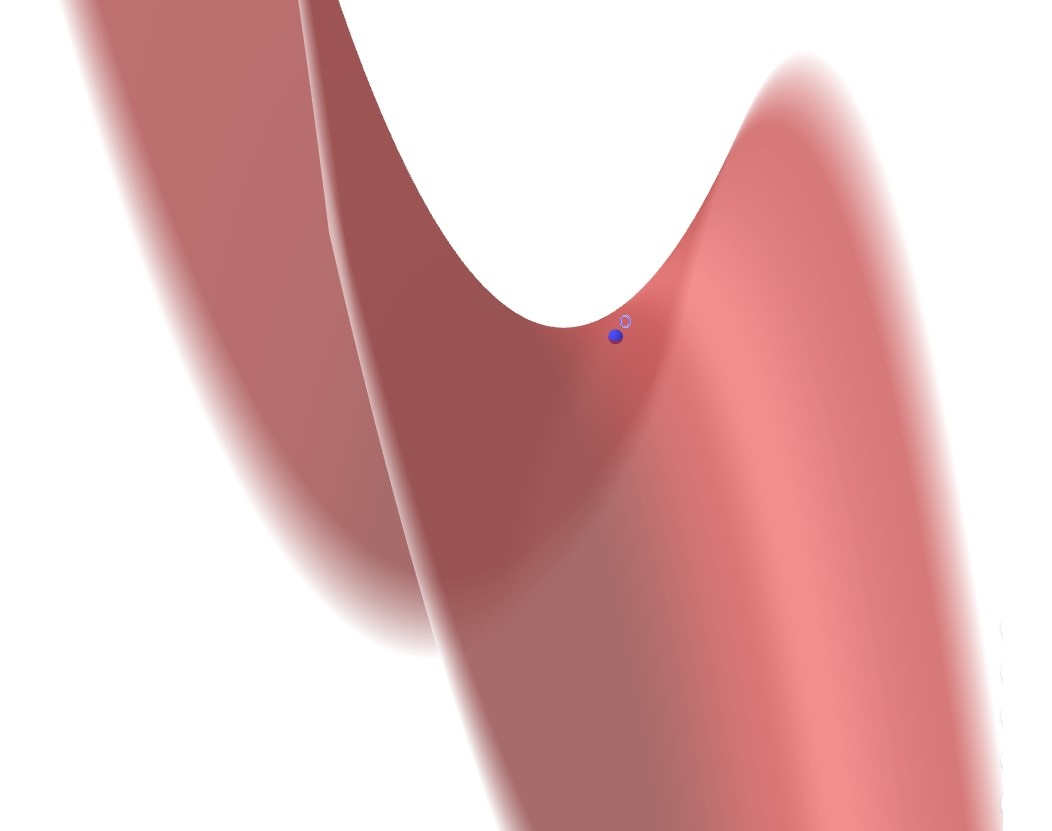
\includegraphics[width=5cm,height=5cm]{C8.jpg}}
        \caption{Punto silla en\\ $z=x^2-y^2$}
        \label{fig:punto_silla}
    \end{figure}
\end{minipage}
\end{nota}

\begin{ejemplo}
    Dada la función $f(x,y)=x^2+xy+y^2$, encontrar sus puntos críticos y clasificarlos.
\end{ejemplo}

\textbf{Solución:}
\begin{itemize}
    \item Primero, calculamos las derivadas parciales de primer orden, esto nos permitirá encontrar los puntos críticos:
    \[
    \frac{\partial f}{\partial x} = 2x + y, \quad \frac{\partial f}{\partial y} = x + 2y
    \]
    \item Para encontrar los puntos críticos, igualamos ambas derivadas parciales a cero:
    \[
    2x + y = 0, \quad x + 2y = 0
    \]
    \item Resolviendo el sistema de ecuaciones:
    \[
    y = -2x, \quad x + 2(-2x) = 0 \implies x - 4x = 0 \implies -3x = 0 \implies x = 0
    \]
    \item Por lo tanto, $y = -2(0) = 0$.
    \item El único punto crítico es $(0,0)$ (otro método más rápido, es observar que se trata de rectas que se intersectan en el origen).
    \item Ahora, calculamos las derivadas parciales de segundo orden, esto nos permitirá clasificar el punto crítico:
    \[
    f_{xx} = 2, \quad f_{yy} = 2, \quad f_{xy} = 1
    \]
    \item Calculamos $D$:
    \[
    D = f_{xx}f_{yy} - (f_{xy})^2 = (2)(2) - (1)^2 = 4 - 1 = 3 > 0
    \]
    \item Dado que $D > 0$ y $f_{xx} > 0$, concluimos que $f$ tiene un mínimo relativo en el punto $(0,0)$.
\end{itemize}

\begin{ejemplo}
    Dada la función $f(x,y)=x^3+y^3-3x-3y$, encontrar sus puntos críticos y clasificarlos.
\end{ejemplo}

\textbf{Solución:}
\begin{itemize}
    \item Primero, calculamos las derivadas parciales de primer orden, esto nos permitirá encontrar los puntos críticos:
        \[
        \frac{\partial f}{\partial x} = 3x^2 -3, \quad \frac{\partial f}{\partial y} = 3y^2 -3
        \]
    \item Para encontrar los puntos críticos, igualamos ambas derivadas parciales a cero:
     \begin{align*}
        3x^2 -3 &= 0, &\quad 3y^2 -3 &= 0\\
        x^2 &= 1, &\quad y^2 &= 1\\
        x&= \pm 1 &\quad y &= \pm 1
     \end{align*}
     \item Por lo tanto, los puntos críticos son $(1,1), (1,-1), (-1,1), (-1,-1)$.
     \item Ahora, calculamos las derivadas parciales de segundo orden, esto nos permitirá clasificar el punto crítico:
    \[
    f_{xx} = 6x, \quad f_{yy} = 6y, \quad f_{xy} = 0
    \]
    \item Calculamos $D$ para cada punto crítico:
    \begin{table}[H]
    \centering
    \begin{tabular}{|c|c|c|c|c|}
    \hline
    Punto crítico & $f_{xx}(a,b)$ & $f_{yy}(a,b)$ & $D$ & Conclusión \\
    \hline
    $(1,1)$ & $6$ & $6$ & $36 > 0$ & Mínimo relativo \\
    \hline
    $(1,-1)$ & $6$ & $-6$ & $-36 < 0$ & Punto de silla \\
    \hline
    $(-1,1)$ & $-6$ & $6$ & $-36 < 0$ & Punto de silla \\
    \hline
    $(-1,-1)$ & $-6$ & $-6$ & $36 > 0$ & Mínimo relativo \\
    \hline
    \end{tabular}
     \caption{Clasificación de los puntos críticos de $f(x,y)=x^3+y^3-3x-3y$.}
     \label{tab:clasificacion_puntos_criticos}
    \end{table}
\end{itemize}

\newpage
\begin{ejemplo}
    Dada la función $f(x,y)=xe^{-x^2-y^2}$, encontrar sus puntos críticos y clasificarlos.
\end{ejemplo}

\textbf{Solución:}

\begin{itemize}
    \item Primero, calculamos las derivadas parciales de primer orden, esto nos permitirá encontrar los puntos críticos:
    \begin{align*}
        \frac{\partial f}{\partial x} &= e^{-x^2-y^2} - 2x^2e^{-x^2-y^2}, &\quad \frac{\partial f}{\partial y} &= xe^{-x^2-y^2}(-2y)\\
        \frac{\partial f}{\partial x} &= (1- 2x^2)e^{-x^2-y^2}, &\quad \frac{\partial f}{\partial y} &= -2xye^{-x^2-y^2}
    \end{align*}
    \item Para encontrar los puntos críticos, igualamos ambas derivadas parciales a cero:
     \begin{align*}
        (1- 2x^2)e^{-x^2-y^2} &= 0, &\quad -2xye^{-x^2-y^2} &= 0\\
        1- 2x^2 &= 0, &\quad -2xy &= 0\\
        x^2 &= \frac{1}{2}, &\quad xy &= 0\\
        x &= \pm \frac{1}{\sqrt{2}}, &\quad y = 0 &\vee x=0
    \end{align*}
    \item Pero ya vimos que $x=\pm \frac{1}{\sqrt{2}}$, entonces no es posible que $x=0$.
    \item Por lo tanto, los puntos críticos son $(\frac{1}{\sqrt{2}},0), (-\frac{1}{\sqrt{2}},0)$.
    \item Al aplicar el criterio de la segunda derivada, se obtiene:
    \begin{table}[H]
    \centering
    \begin{tabular}{|c|c|}
    \hline
    Punto crítico & Conclusión \\
    \hline
    $(\frac{1}{\sqrt{2}},0)$ & Máximo relativo \\
    \hline
    $(-\frac{1}{\sqrt{2}},0)$ & Mínimo relativo \\
    \hline
    \end{tabular}
     \caption{Clasificación de los puntos críticos de $f(x,y)=xe^{-x^2-y^2}$.}
     \label{tab:clasificacion_puntos_criticos_2}
    \end{table}

    %  \item Ahora, calculamos las derivadas parciales de segundo orden, esto nos permitirá clasificar el punto crítico:
    % \begin{align*}
    %     f_{xx} &= \frac{\partial}{\partial x}\left((1- 2x^2)e^{-x^2-y^2}\right)\\
    %     &= -4xe^{-x^2-y^2} + (1- 2x^2)(-2x)e^{-x^2-y^2}\\
    %     &= (-4x + 2x - 4x^3)e^{-x^2-y^2}\\
    %     &= (-2x - 4x^3)e^{-x^2-y^2}
    % \end{align*}
    % \begin{align*}
    %     f_{yy} &= \frac{\partial}{\partial y}\left(-2xye^{-x^2-y^2}\right)\\
    %     &= -2xe^{-x^2-y^2} + (-2xy)(-2y)e^{-x^2-y^2}\\
    %     &= -2xe^{-x^2-y^2} + 4xy^2e^{-x^2-y^2}\\
    %     &= (-2x + 4xy^2)e^{-x^2-y^2}
    % \end{align*}
    % \begin{align*}
    %     f_{xy} &= \frac{\partial}{\partial y}\left((1- 2x^2)e^{-x^2-y^2}\right)\\
    %     &= (1- 2x^2)(-2y)e^{-x^2-y^2}\\
    %     &= (-2y + 4x^2y)e^{-x^2-y^2}
    % \end{align*}
    % \item Calculamos $D$ para cada punto crítico:
    % \begin{table}[H]
    % \centering
    % \begin{tabular}{|c|c|c|c|c|c|}
    % \hline
    % Punto crítico & $f_{xx}(a,b)$ & $f_{yy}(a,b)$ & $f_{xy}(a,b)$ & $D$ & Conclusión \\
    % \hline
    % $(\frac{1}{\sqrt{2}},0)$ & $-2\sqrt{2}e^{1/2}$ & $-2\frac{1}{\sqrt{2}}e^{1/2}$ & 0 & (+) & máximo \\
    % \hline
    % $(-\frac{1}{\sqrt{2}},0)$ & $2\sqrt{2}e^{1/2}$ & $2\frac{1}{\sqrt{2}} - 4(-\frac{1}{\sqrt{2}})^2 \cdot 0$ & 0 & (+) & mínimo \\
    % \hline
    % \end{tabular}
    %  \caption{Clasificación de los puntos críticos de $f(x,y)=xe^{-x^2-y^2}$.}
    %  \label{tab:clasificacion_puntos_criticos_lagrange}
    % \end{table}
\end{itemize}

\newpage
\section{Método de multiplicadores de Lagrange}